\documentclass[a4paper, 12pt]{article}
\usepackage[utf8]{inputenc}
\usepackage[margin=0.9in]{geometry}
\usepackage{graphicx}
\usepackage{textcomp}
\usepackage{setspace}
\usepackage{hanging}
\usepackage{listings}
\usepackage{pdflscape}
\usepackage[english]{babel}
\usepackage[nottoc]{tocbibind}
\usepackage{lmodern}
\usepackage{csquotes}
\usepackage[backend=biber,style=authoryear]{biblatex}
%\usepackage[style=apa]{biblatex}
\DeclareLanguageMapping{british}{british-apa}
\renewcommand{\figurename}{Example}
\addbibresource{GP.bib}
\usepackage{hanging}


\begin{document}
\begin{titlepage}
\addtolength{\hoffset}{0cm}
	\centering
	
\includegraphics[width=0.90\textwidth]{monash1line.jpg}\par\vspace{2cm}
	{\LARGE\bfseries A data mining technique to detect coronary artery disease using hybrid predictive modelling \par}
	\medskip\medskip
	\hrule
	\vspace{3cm}
	{\Large\bfseries Yupeng (Vita) Miao \par
	\medskip
	Yunxuan Wang \par
	\medskip
	Chang Yu Wang \par}
    \vspace{3cm}
    
   {\Large\bfseries Monash University\\}
    \medskip
    \large\textbf{Faculty of Information Technology\\}
    
    \vspace{3cm}
     % Bottom of the page
	\large{A Project Proposal for \textit {FIT3163}}\\
	\vspace{2cm}
	Word count: 7204\\
	\vfill
	{\large  June 2020}
\end{titlepage}
\onehalfspacing
\tableofcontents
\pagebreak
\onehalfspacing

\section{Introduction}
As the leading cause of death in many developed countries, including Australia, Coronary Artery Disease (CAD) diagnosis is a high priority. In 2017, it accounted for 11.5\% of all deaths in Australia (18590), and is especially prevalent in the elderly population aged 45 and over (AIHW, 2019). The current leading method of diagnosing CAD is angiography, which is both invasive and expensive. We aim to circumvent this by creating a model to aid medical professionals diagnose CAD using non- or minimally- invasive patient information. This model would take features such as the height, weight, and family history of a patient, as well as results from a simple blood test such as potassium or triglyceride content in the blood. It will be built using hybrid predictive modelling on a variety of well-known classifier methods from data science. 
\\\\
The model is to be built in R using an assortment of packages and libraries. It will then be hosted as a public API and a simple website will be created to allow all users to interact with it. In the coming months and throughout semester 2, we will clean the data, and build the model in a four-stage approach. The first stage will consist of preliminaries, such as wrangling the data and learning about methods for future stages, such as classifier algorithms or web design. Stage two involves training an assortment of singular models, selecting the best performing for the next stage. Stage three will take these models and combine them into hybrid models with a variety of approaches, iterating where possible. This will include comparing and contrasting the results. The best performing hybrid model will be hosted as the API. Finally, we will create the API, website, and all related documents in the fourth stage.

\section{Literature review}
    \subsection{Literature Review Introduction}
    Data mining is an emerging field in the healthcare industry as it has shown great potential in helping doctors make more accurate and efficient disease diagnosis (Shamsollahi, Badiee, \& Gahazanfari, 2019). The medical diagnosis for CAD is extremely important in practice, however, traditional diagnosis methods are based on doctors’ experiences. They require the patients to undergo various expensive tests, making the diagnosis a rather complex task (Shamsollahi et al., 2019). With the help of data mining, doctors can more easily make efficient and accurate CAD diagnosis (Mustafa, Saeed \& Jasim, 2018). Furthermore, a smart CAD prediction system would also give the patients a warning about the conceivable likeness of CAD even before taking the costly check-ups in the hospital (Mathan, Priyan, Panchatcharam, Manogaran, \& Varadharajan, 2018). This section presents a comprehensive review of recent studies on CAD diagnosis with a data mining approach. This review aims to gain a deeper understanding of this topic and observe anything worth considering in our project.\\\\
    Researchers have proposed many different data mining approaches for CAD prediction and some of the popular works are examined here. To ensure the objective reliability of the sources, we conduct a CRAPP test, a widely used test in the academic discipline for source evaluation. The studies that have been reviewed in this section cover related works in the last ten years as the exploration of using data mining for disease diagnosis only took off around 2010. Moreover, all the papers are peer-reviewed journal articles, which guarantees the information used is trustworthy.\\\\
    Most early studies focus on developing classifiers for CAD diagnosis using single machine learning techniques and identifying the most effective feature selection approach, while more current research targets proposing a hybrid classification model for coronary illness prediction. The following aspects are presented in the literature review: section 2.2 presents the data mining tools that are were used in previous studies, section 2.3 indicates the dataset that has been widely used for CAD prediction, section 2.4 discusses the data wrangling techniques implemented by related studies, section 2.5 presents the effective algorithms for feature selection within the context of CAD, and finally, section 2.6 details the hybrid strategies proposed by recent research.

    \subsection{Data Mining Tools}
    Data mining procedures refer to the techniques for model fitting and are currently in a phase of rapid advancement, while a wide variety of data mining tools, such as MATLAB, are also available for free. This allows researchers the ability to utilize any tool they prefer to facilitate the data mining implementation (Toigui, Jilbab, \& El Mhamdi, 2020). Tougui et al. (2020) compared six different data mining tools that can be used for CAD prediction on six classification techniques. Amongst MATLAB, Knime, WEKA, RapidMiner, Orange, and Scikit-Learn, MATLAB achieved the best overall performance, especially with Artificial Neural Networks (ANN) where it obtained an accuracy of 85.86\%. Moreover, for users with different levels of experience in data mining, Tougui et al.’s research (2020) also provides recommendations on choosing the most suitable data mining tool. 
    \\\\
    Orange does not give the users much control over data mining algorithms but offers a user-friendly interface; hence being recommended for researchers with minimal data mining knowledge. Researchers with a good understanding of machine learning techniques can be benefit from using Knime or RapidMiner since these two tools allow users to manipulate the parameters of various techniques (Toigui et al., 2020). Several related studies employ RapidMiner 5 to implement their proposals (Bashirm, Qamar, \& Kahn, 2016), and the advantages of using RapidMiner have been highlighted by Bashir et al. (2016): that it supports effective functionality and open source innovation, and its virtual design environment is easy-to-use but robust.
    \\\\
    MATLAB allows for data wrangling and is a tool that our group can consider using due to it being particularly recommended for people with strong programming skills (Toigui et al., 2020). However, Tougui et al.’s research did not discuss other popular tools such as R or Python and hence this research cannot be considered as conclusive. The performance of these data mining tools may also vary with different datasets or features, and thus, evaluating performance on other datasets is required for robust results. 
    \\\\
    R Studio is also a popular tool in data mining and has been used in several CAD prediction studies (Gupta, Ahuja, Malhotra, Bala, \& Kaur, 2017 and Vijayashree \& Sultana, 2018), there exists an enormous amount of open-sourced R packages to support the researches to facilitate their data mining application, including the data wrangling process. The data pre-processing can be done in different software, such as SPSS or Excel Vijayashree \& Sultana, 2018).
    \\\\
    Cloud computing is emerging as a competitor in many fields as it supports the analysis of the large datasets. To investigate the performance of a cloud platform, (Gupta et al., 2017) implements data mining techniques for CAD diagnosis using Hadoop on Amazon EC2, comparing the accuracy and analysis time to that of applying algorithms using R. The results suggest that the higher accuracy is achieved by implementing machine learning techniques in the cloud environment with slightly lower standard deviation and less execution time. The advantages of cloud-based data mining are highlighted when the dataset is huge, as the difference in efficiency between the cloud model and standalone machine model increases as the size of the dataset increases. However, to our knowledge, none of the published datasets about CAD has a size greater than 500 and so the benefit of using the cloud platform may not be significant in our project. The cloud-based approach can be considered when more medical data about CAD is available.
    
    \subsection{The Dataset}
    Eleven out of nineteen studies reviewed have used the Cleveland Clinic Foundation database from UCI repository either as the training dataset or a dataset for validation, as it is free from missing values and has little noisy data (Mathan et al., 2018, Gupta, Ahuja, Malhotra, Bala, \& Kaur, 2017, and Dwivedi, 2018.). As this classic dataset contains 303 observations and only 13 attributes, the Statlog dataset and other heart disease datasets from UCI repository are often combined with the Cleveland dataset for model training (Bashir et al., 2016). Vijayashree \& Sultana (2018) and Gupta et al. (2017) have also used additional data that is not accessible to the public from other medical health institutes. Our project can benefit from using the Cleveland database since we can then easily compare the performance of our proposed models to the models implemented by other researchers using the same dataset. 
    \\\\
    Nevertheless, Z-Alizadeh et al. (2012) claim that the most frequently used datasets from the UCI repository are no longer up-to-date, and their team constructed a new dataset for future studies in CAD prediction. Unfortunately, the sizes of these medical datasets are relatively small and contain different sets of attributes, which means that they cannot be combined easily. Therefore, sampling with repetition techniques, such as bootstrapping, should be considered to reduce the biases. \\\\
    
    \subsection{Data Wrangling Techniques}
    Mathan et al. (2018) emphasized in their research that the appropriate data pre-processing is crucial for achieving the full potential of data mining techniques because the redundancy and inconsistency that exists in the raw medical dataset would affect the prediction performance of machine learning techniques. The data wrangling steps, such as missing value imputation, outlier detection, attributes normalization, and removal of noisy data, are followed by many of the studies that have been reviewed in this section (Bashir et al., 2016). In particular, (Bashir et al., 2016) adopted the binning technique to remove noisy data. A similar approach for data wrangling is likely to be followed in our project to advance the performance of our models. However, a more systematic analysis of data wrangling techniques in CAD prediction is needed to highlight the significance of applying data wrangling techniques in improving the CAD prediction performance with data mining approaches.
    
    \subsection{Feature Selection Strategies}
    Several studies suggest that the effective use of feature selection techniques is required to advance the CAD prediction accuracy and computational efficiency (Tarawneh \& Embarak, 2019), since the attributes that do not contribute significantly to the CAD prediction can weaken the performances of the data mining models 17. Dinesh et al. (2018) proposes a remarkable feature selection framework with Improved Particle Swarm Optimization for CAD prediction, which is compared with ten other popular feature selection techniques: PSO, Info gain, Filtered attribute, Filtered subset, Chi squared, Gain ratio, Relief, Consistency subset, CFS and One attribute based. 
    \\\\
    The framework incorporates the original PSO and SVM with an optimal weights identification function that helps to update the position of the articles (Vijayashree \& Sultana, 2018). The original PSO algorithm has trouble with obtaining the ideal weights to update the particle position, while the proposed framework overcomes this with the help of the novel function presented. As a result, the SVM classifier using this proposed framework obtains an accuracy of 84.36\%, outperforming models with other feature selection techniques (Vijayashree \& Sultana, 2018). This result should be tested on different datasets using various classification algorithms, but nevertheless, is still a remarkable feature selection approach that our project can follow.
    \\\\
    Various other feature selection approaches are followed by researchers. Tarawaneh \& Embarak (2019) evaluated a few popular feature selection techniques and they yield on the same conclusion that SVM achieves the most outstanding performance in CAD prediction. Moreover, it is suggested by Gupta et al. (2017) that the correlation analysis of the attributes will help to eliminate any insignificant features in CAD prediction, as the highly correlated attributes are not going to play important roles in the classification. Since the correlation analysis is relatively easy to implement, our project can consider using this technique to simplify our model without losing information. The all-subset approach is adopted by Jha et al. (2019) testing 8100 combinations of the features to obtain the nine most significant features in CAD prediction. It is applicable because the dataset they used only contains 13 attributes, but when the number of attributes increases, such as the Z-Alizadeh Sani dataset which includes 54 attributes, this approach is no longer appropriate as it would require too much computation time. 
    
    \subsection{Classifier Hybridization Strategies} \label{Hybrid_strategy}
    Classifiers with single machine learning techniques have been compared by many prior studies (Vijayashree \& Sultana, 2018, Dinesh et al, 2018), highlighting the significance of Logistic Regression, SVM and ANN in CAD prediction. Instead of using a single machine learning algorithm for classification, the latest studies in CAD prediction use a data mining approach proposing several hybrid frameworks which aggregate the results from various nominal classifiers (Mathan et al., 2018, Bashir et al., 2016, Gupta, Ahuja, Malhotra, Bala, \& Kaur, 2017). The overall performance of these hybrid models are showed to be better than other classifiers using single machine learning techniques.
    \\\\
    The most common technique for model aggregation is combining results from different models using voting schemes (Bashir et al., 2016). Bashir et al. (2016) presents an ensemble model that combines five distinct nominal classifiers by weighted vote-based techniques for CAD prediction. The five classifiers are the decision tree based on information gain, instance-based learner (IBL), decision tree based on Gini index, Naive Bayes, and the SVM, covering both lazy and eager classification algorithms. Through aggregating lazy and eager classifiers, this proposed framework overcame each of their limitations and achieves a remarkable accuracy of 87.37\%. This proposed model has been tested on five different datasets to ensure the robustness of the result. However, the hybrid model has only been compared to each of the individual classifiers in the hybrid model, thus, additional studies to compare the hybrid model with other nominal classifiers and hybrid models are required to identify the most effective classification framework for CAD prediction. 
    \\\\
    The promising results of CAD prediction achieved by hybrid models are further evidenced by Gupta et al. (2017). Rather than predetermining the classifiers to be combined like in Bashir et al. (2016), Gupta et al. (2017) first trained seven distinct classifiers and then combined the top three performed classifiers to form the hybrid model, this methodology is likely to obtain a greater improvement in CAD prediction than that of Bashir et al. (2016). The final hybrid model incorporates the Naïve Bayes, AdaBoost, and Boosted tree, where Naïve Bayes obtained the highest accuracy of 86.42\% among all seven algorithms tested. The hybrid model boosted the accuracy to 87.91\%, although the improvement made is relatively small, it shows greater stability over the nominal classifiers. Another remarkable hybrid model combined with seven nominal classifiers using voting techniques is proposed by Tarawaneh \& Embarak (2019), which presents an accuracy of 89.2\%. However, it seems that a common problem in using hard voting is that the hybrid models are not able to predict the intensity of CAD. One way to overcome this problem is by using fuzzy learning models which can determine the intensity of the CAD.
    \\\\
    Another common approach for aggregation involves combining descriptive and predictive algorithms of data mining for CAD prediction (Shamsollahi et al., 2019).  The Shamsollahi et al. (2019) study first divided up the dataset using a descriptive method, k-means clustering, where the number of clusters, k, is predetermined based on several indices including the Dunn index, elbow algorithm, and the gap statistic method. In order to obtain the optimal predictive results, Shamsollahi et al. (2019) then applied five predictive methods (CHAID, C\&RT decision tree, ANN, C5.0, and Quest) to each of the clusters. Among all the combinations trained by Shamsollahi et al. (2019), k-means clustering with the C\&RT decision tree achieved the best prediction result with prediction error at only 0.074. 
    \\\\
    To validate the performance, these models were then tested on 17 benchmark healthcare datasets. However, the proposed model uses the same classifiers on all clusters and, if we take a closer look at each individual cluster, the optimal results are achieved by different classification algorithms. Therefore, a potential solution to further advance this proposed framework is to fit different classifiers for each of the clusters, and also test other combinations of descriptive and predictive methods for CAD prediction. Moreover, a similar hybrid model was presented by (Mohan, Thirumalai \& Srivastrava, 2019), using a random forest trained for data partitioning and then a logistic regression for estimating each cluster. This hybrid random forest with a linear model (HRFLM) boosts the predictive performance with an accuracy of 88.7\%. Since the Monan et al. (2019) study used the entire set of attributes, one way of further enhancing this proposed hybrid model is to eliminate any insignificant features by implementing proper feature selection techniques.\\
    \\
    There are also several studies focusing on advancing particular machine learning algorithms for CAD prediction. The genetic algorithm is applied by Krishnaiah et al. (2015) to enhance the performance of the ANN classifier. The results suggest that through determining better initial weights of neural networks with the help of a genetic algorithm, the ANN for CAD prediction can find a better minimum and increases performance by approximately 10\% obtaining a remarkable accuracy of 93.85\%. Future studies can try other techniques in this manner instead of using the genetic algorithm, such as evolutionary and PSO, to improve the performance of the neural network in CAD prediction. In addition, other techniques, such as the discretization strategy (Mathan et al., 2018) and fuzzy learning method (Krishainah, Narsimha \& Chandra, 2015), have also been implemented to enhance the performance of classification algorithms.
    
    \subsection{Literature Review Conclusion}
    To conclude, there are some techniques that we find worthwhile to learn from as well as a few common limitations to the prior studies. Most of the prior studies are based on small but classic CAD datasets which may introduce biases into the model training. As our project will likely to use these classic datasets, we can validate our models through testing them on various other datasets to ensure our models are robust. Second, the analysis about computation time is not included in the performance evaluation for many of the studies, while the efficiency can be an important benchmark for performance measurement. Some of the data wrangling techniques and feature selection frameworks proposed by the prior studies are worthwhile to consider in our project implementation, such as using binning techniques to remove the noisy data and improved PSO for feature selection. As far as we know, no previous researches have compared different hybrid machine learning models in CAD prediction, our team therefore will analyze various strategies to aggregate classifiers and hence identify the most effective and robust data mining approach for CAD prediction.
\pagebreak    
\section{Project Management Plan}
    \subsection{Project Overview}
    Our key objective is to create and host a hybrid model for aiding CAD diagnosis as a public API. This is broken down into four major work activities.
    \begin{enumerate}
        \item Wrangle data and upskill team members, ensuring adequate knowledge of modelling methods, GitHub, and web design.
        \item Create a strong collection of singular classifiers for CAD.
        \item Combine the singular classifiers into an assortment of hybrid classifiers, selecting the strongest performing hybrid model.
        \item Host this result an API and create a website to access the model.
    \end{enumerate}
    \begin{figure}
        \centering
        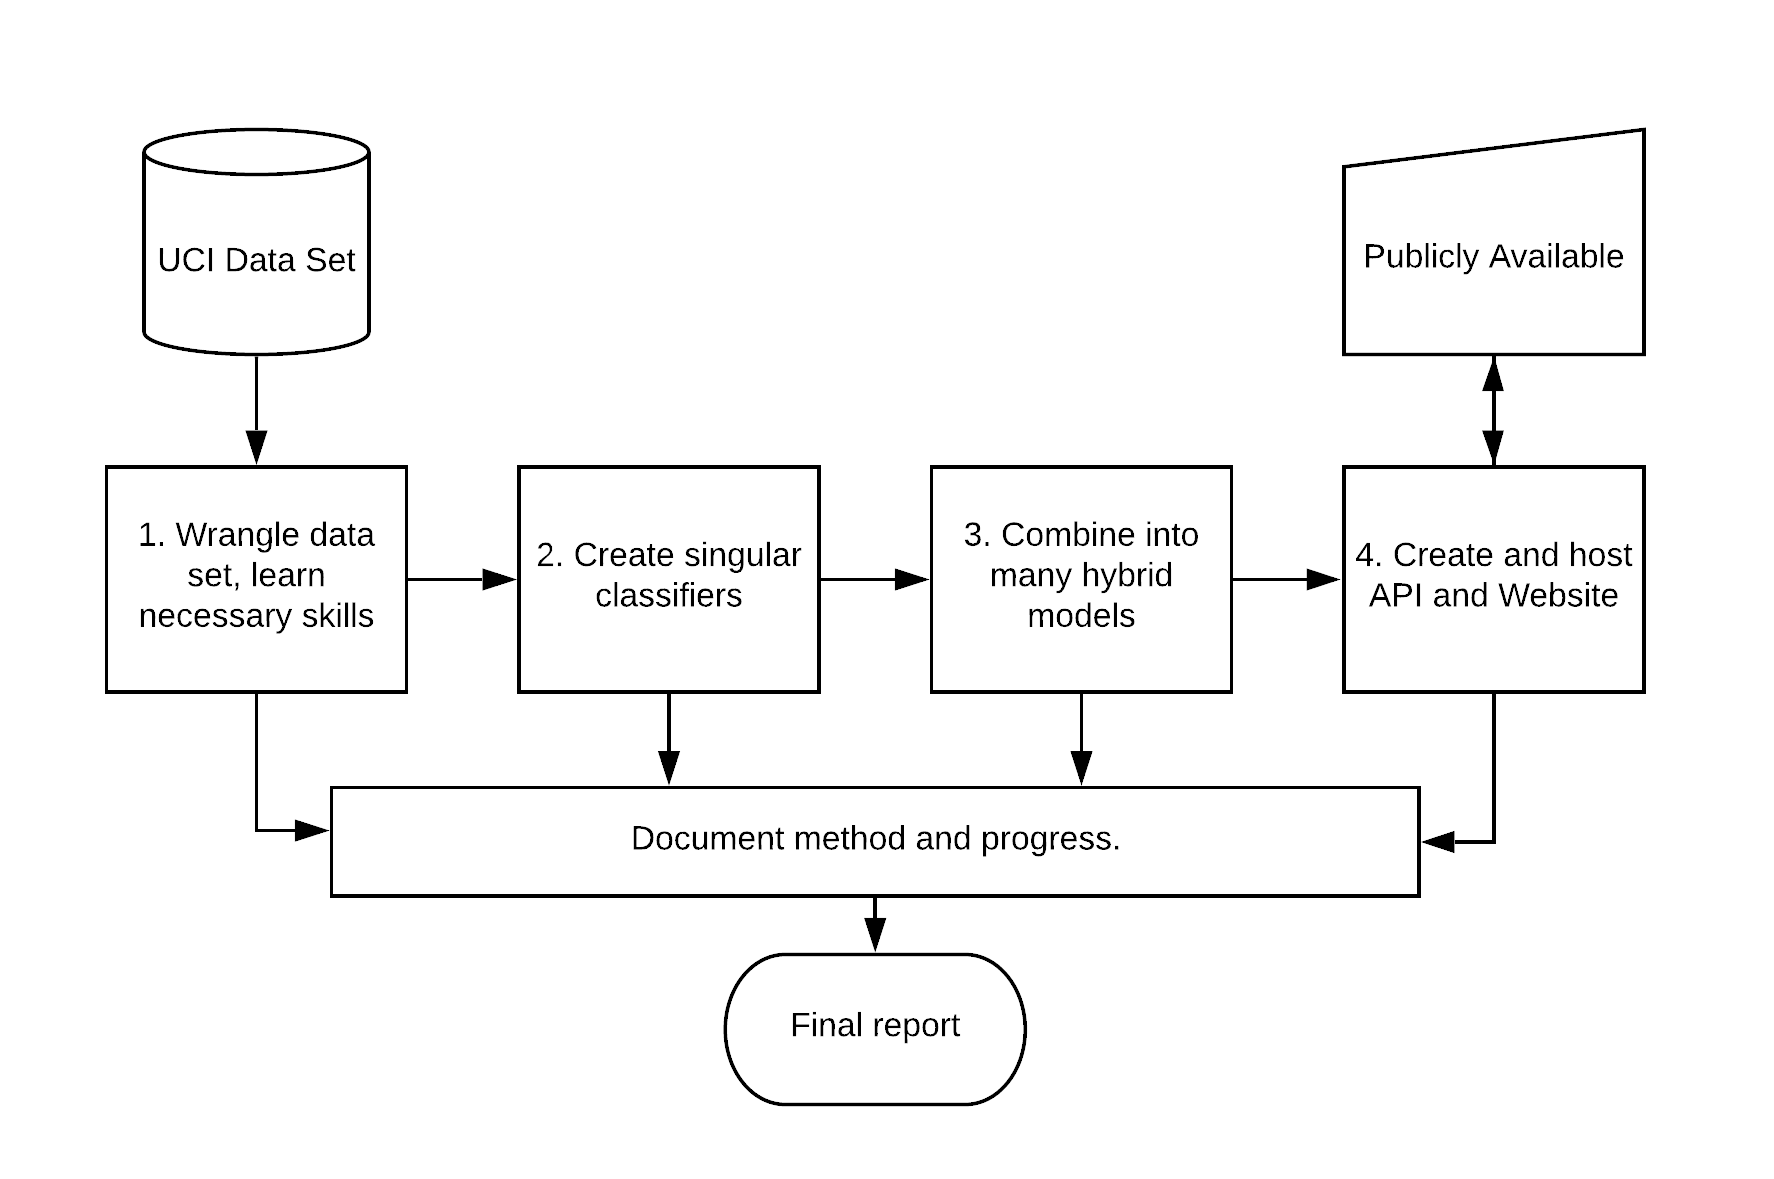
\includegraphics[width=0.8\textwidth]{FIT3163 Project Milestones.png}
        \caption{The key milestones for our project. We will be continuously documenting the process.}
        \label{fig:milestones}
    \end{figure}
    \subsection{Project Scope}
        \subsubsection{Project Deliverables} \label{deliv}
        The key deliverables for this project are:
        \begin{enumerate}
            \item A hybrid model for diagnosing CAD
            \item A publicly hosted API
            \item A simple website to allow users to access the API
            \item User guides and related documentation
            \item Project Management related documents: Project Proposal, WBS, RTM, Risk Breakdown Structure, Status reports, Lesson-learned reports, and other related documents.
        \end{enumerate}
        These align with, and will be completed by, stages 3 and 4 of the project plan.
        
        \subsubsection{Project Characteristics and Requirements}
        The project is to satisfy the following requirements.
        \begin{enumerate}
            \item To be completed by the end of Monash University's Semester 2, 2020.
            \begin{enumerate}
                \item The work is to be split equally between all team members.
                \item The project is not paid, and any costs are to be covered personally.
            \end{enumerate}
            \item Create a model that takes in values for specific features, and gives a prediction on the presence of CAD.
            \begin{enumerate}
                \item We note that we are not medically trained, and that results are not a substitute for professional advice.
                \item The model is to be a hybrid of many different individual classifiers that are well known in the data science sphere.
                \item The hybrid model should perform better than all component models.
                \item The methods to build the model are to be based on insight gained from the literature review.
            \end{enumerate}
            \item The API and website should be publicly available and stay online for at least a year. It should support a small number of concurrent users (5+), and be scale-able if the need arises.
            
            \item There is no need for data storage, as the training data is small and can be embedded into the API. User data from the website will also not be stored.
            \item There will be a developer manual for how to access the features that the API provides. The website will also have a quick user guide, which includes interpretation of the results.
            \item All governing processes and documents for the duration of the project are to be stored and available upon request.
            \begin{enumerate}
                \item Governing documents include the Requirements traceability matrix, risk register, and work breakdown structure.
                \item Other documents include meeting minutes, Lesson-learned reports, and progress updates.
            \end{enumerate}
        \end{enumerate}
        
        \subsubsection{Produce User Acceptance Criteria} \label{Acceptance_Critera}
        \begin{enumerate}
            \item The website and API should be published and available for use by the end of semester 2, 2020.
            \item The model should give an accurate prediction of the presence of CAD, to aid in a medical professional's diagnosis.
            \item Users of the API should be able to send a request by providing a set of values (or N/A) for given variables. The API should then respond with a suggested diagnosis of CAD. This response should be as accurate as possible, comparable to non-data science approaches.
            \item The website should allow users with no technical ability to send a request to the API. It should be efficient and easy to use. Users can manually input the values into a set of boxes on the website, and the result should be displayed clearly. Specifics are mentioned in the external design section (section \ref{extdes}).
            \item Associated graphs for visualisation of risk should also be accessible from the website.
            \item If interested, a user should be able to learn how to use the website and API from the provided documentation and user guide.
        \end{enumerate}

    \subsection{Project Organisation}
        \subsubsection{Process Model}
        We will begin with a predictive approach for stages one and two, as the the initial steps are quite rigidly defined - wrangle the data and build an assortment of predictive models. This will allow the team to make rapid progress without interruption, as the aims are not likely to change. We are also more familiar with these methods, owing to previous projects in earlier studies.
        \\\\
        Then, as the project approaches more uncertain material in stage three, we will move to an agile approach. This will help us create and evaluate the new hybrid models, as well as tackle the challenges that arise with creating and hosting the API and website. An agile approach here is more appropriate here as the approaches to combining models are unfamiliar and will require many iterations to improve the final result. The agile methodology is also advantageous approaching the deadline, as we can ensure the most important requirements are met. %maybe diagram here
        
        \subsubsection{Project Responsibilities} \label{model_respon}
        Yunxuan will wrangle the data whilst others read up on any necessary material, such as background on new classifiers or how to use GitHub.
        \\\\
        Then, all team members are responsible for the technical functionality in the project: training the component models in the second phase and hybrid models the third phases. 
        \\\\
        In stage 2, the component models will be divided up based on familiarity with the classifier.
        \begin{itemize}
            \item Chang - Support vector machines, Quadratic Discriminant Analysis, Bayesian linear regression. 
            \item Vita - Random forests, Neural Networks, K-means clustering.
            \item Yunxuan - Naive Bayes, K-nearest neighbours, Logistic Regression.
        \end{itemize}
        
        Then the hybrid model building phase (stage 3) will be led by Vita, including leading the scrums for agile development and identifying the methods and approaches that are most effective. Chang will be responsible for the API and website development stage (stage 4) and related functionality, choosing and hosting the resulting products and writing the user guides. This includes meeting the website functionality specified in the User Acceptance Criteria and External Design sections (\ref{Acceptance_Critera} and \ref{extdes} respectively).
        \\\\
        Yunxuan will oversee the non-technical requirements. This includes the ongoing scheduling, managing of resource requirements and timelines of the project. This also includes creating the required management documents, user guides and documentation. 
        \\\\
        As leads, each team member will delegate tasks to the others to ensure equal contribution, development-wise. Finally, all written submissions and documents will be equally divided up, with Chang serving as the quality assurance manager.
        
    \subsection{Management Process}
        \subsubsection{Risk Management Process}
        Our risk management plan identifies and details responses to potential risks throughout the project, and all members will be familiar with the avoidance and acceptance strategies proposed. We initially held group brainstorming sessions to generate an extensive list of potential risks. Then, we applied SWOT analysis to identify all strengths, weaknesses, opportunities, and threats.
        After the SWOT analysis, we summarised the results into a risk register attached in the appendix. 
        \\\\
        Then we used a probability/impact matrix as qualitative risk analysis tool, listing the relative probability of the risk occurring on one side of our matrix and the relative impact of the risk occurring  on the other side. To mitigate the effect of negative risks, we applied the TARA principle to our plans, evaluating whether we should Transfer, Avoid, Reduce, or Accept the risk and created contingency plans. We will also schedule buffer times throughout the project, so that we can deal with any unknown risks.
        \\\\
        We also have tried to maximise the effect of identified positive risk without negatively affecting our workflow, by aiming to maximise the cost-benefit of any enhancing method.
        
        \subsubsection{Monitoring and Controlling Mechanisms}
        We will evaluate the project performance through weekly meeting and consultations with our supervisors. We will take corrective actions if we find any unidentified risks or if we differ from the plan. We will follow and update the requirements traceability matrix and create progress reports help us to monitor the project.
        
        \subsubsection{Communication and Reporting plan}
        We will have weekly meetings on Zoom, as a status report on tasks completed, to plan the coming week's tasks, as well as provide feedback and advice. Here, we can bring up any difficulties we are having, or reallocate tasks based on the previous week.
        This is supplemented with WeChat and Facebook Messenger for instant informal communication when task requirements change or to otherwise keep each other updated. 
        We will also use email for formal communication. This is to be used when communicating with our supervisors/TAs, as well as anything else formal in nature, such as to create a paper trail for documents (e.g. submission confirmations).
        \\\\
        All meetings will be documented by minutes, which will be posted on the group Google Drive and we will have along with progress reports that detail the current status of the project.
        %Communication table
\begin{figure}[ht]
    \centering
    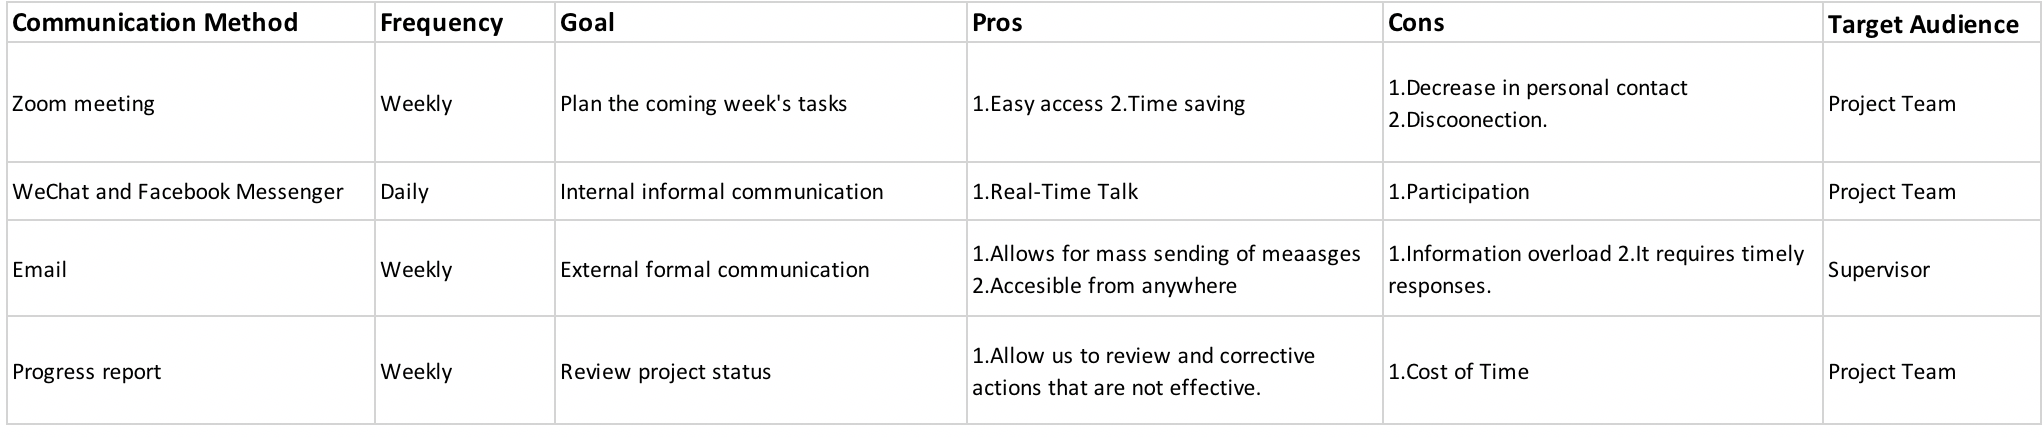
\includegraphics[width=1\textwidth]{Communication Table.png}
    \caption{A communication table summarising our various methods of communication.}
    \label{fig:model_summary}
\end{figure}
        
        \subsubsection{Review and Audit Mechanisms}
        GitHub will be our version control software for code, which will allow for a record of edits made and whom by. This will be vetted if anything unexpected happens, and can be reverted to or merged with at any time. Overleaf and Google Drive will serve as measures for preserving written documents, such as project management related charts and the final submission. Exact details and procedures can be found in the Version Control section under Methodology (\ref{ver_ctrl}).
        \\\\
        Getting feedback from supervisors will be our primary quality assurance tool in the initial stages of the project, for planning related topics such as scope or timeline. As we progress, we will consult the literature to compare the quality of our models, aiming to get at least comparable accuracy.
        We may also create a flowchart to document process flows, so we can locate any breakdowns in our work process. Network diagrams and Gnatt charts will be created and maintained to audit our progress and stay on track.
        \\\\
        Finally, we will conduct a lessons-learned review after every major milestone, in order to consolidate training as well as prepare for the next task. Here, we will test each other's work as a form of quality assurance, and follow steps outlined in section 6, test planning. In this step, we may also identify holes in subject matter, and take time to engage in training. This can take the form of online classes to reading user guides on creating websites.

    \subsection{Schedule and Resource Requirements}
        \subsubsection{Schedule}
        Following the submission of this document, work will begin on data wrangling and model construction. The stages outlined in the introduction will be scheduled as follows.
        The first two phases are to be conducted following the predictive approach and are estimated to take around a month each, with phase one ending mid-July and phase two ending mid-August. These phases have redundancies built in to accommodate for any unknown risks or delays. 
        \\\\
        Then, stages three and four have a less strictly defined schedule, following the agile methodology. While the entire project has a hard deadline at the end of October, the exact distribution of work in these two and a half months can be moved around to suit the needs of the team. Development stages can even be concurrent, to ensure the most important deliverables outlined in (\ref{deliv}) are met.
        \\\\
        Finally, in the last two weeks of October, we will also create any extraneous documentation not completed during the previous months, such as the final report. A network diagram summarising these dependencies is attached in the appendix (Example \ref{fig:dependency}).

        \subsubsection{Resource Requirements}
        With the exception of stage one, all three members should take an estimated 12 hours a week to complete allocated tasks for the project, including the weekly meeting and any discussions with our supervisors. This is equivalent to a full-time unit loading, and is an appropriate amount of time to spend coding, testing, and communicating changes.
        This time also includes any additional study required to complete new tasks.
        \\\\
        Stage one is projected to take significantly less resources, as there is no model training or difficult computation involved. This also falls during the exam period and mid-year break, and so, we have spread out the resources over a longer period of time.
        \\\\
        Regarding software requirements, we will use R studio and associated packages listed in the appendix from the CRAN package repository for all model construction related works. This includes “plumber” to host the API. For Hardware requirements, we need a computer with multi-core processor, RAM at least 8 GB. If any member does not have access to a powerful enough computer to train the models, the code can be run on another team member's computer or on Monash resources.
        \\\\
        All team members must also have the appropriate network requirements, with access to GitHub, Google Drive, Moodle, and one of Facebook messenger or WeChat. This should also suffice for any internet research.
        
\section{External Design} \label{extdes}

   \subsection{Externally Observable Features \& User Interface}
        \subsubsection{External Interface}
Our interface will have input data collection, where users can provide the data required for prediction. This can be in the form of entering values into fields and drop down displays, or just importing a .csv or .xlsx file. This is sent to the API and a result is fetched and displayed on the following page, which shows the predicted result as well as the expected accuracy of the prediction. This expected accuracy is a function of the method testing accuracy, and may also be adapted based on the strength of model locally around the input point. We may also display a graph comparing the user data and comparing it to other entries in the dataset, showing hoe it compares versus patients with and without CAD.
\begin{figure}[ht]
    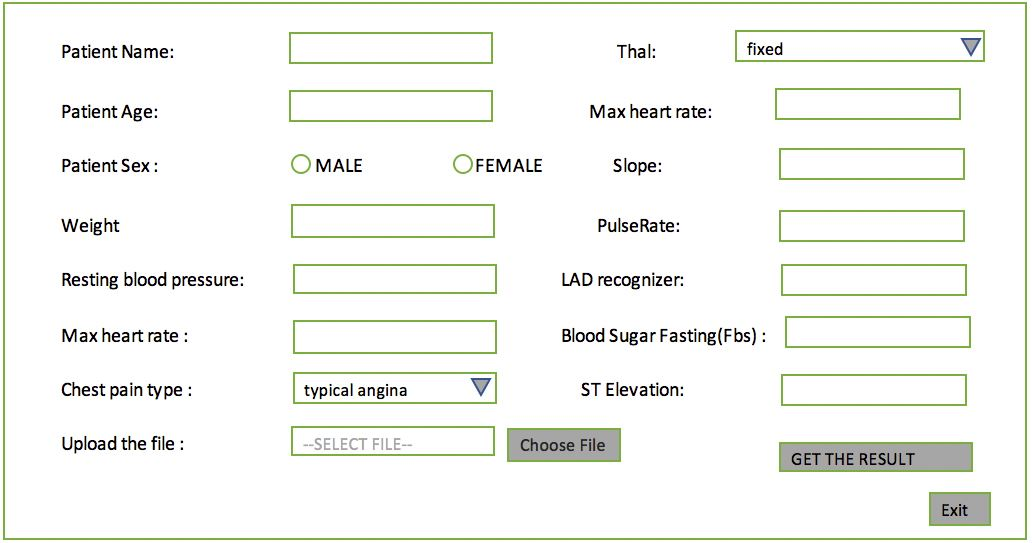
\includegraphics[width=0.501\textwidth]{UI1.JPG}
    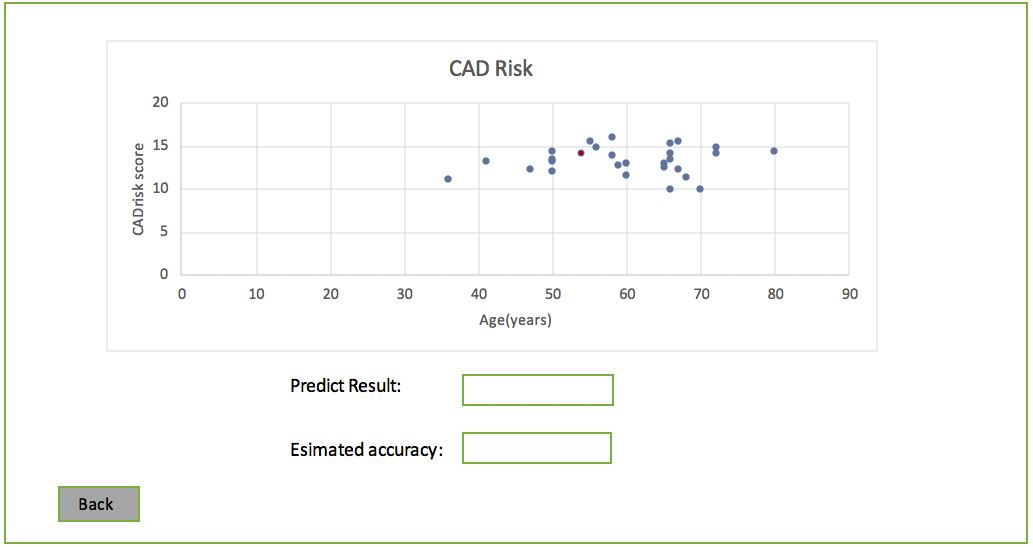
\includegraphics[width=0.498\textwidth]{UI2.JPG} 
    \caption{An example of the user interface. The left-hand figure is the first page that provides boxes for users to input data. Alternatively, they may upload a file instead. The result page is on the right, and displays the predicted result, along with expected accuracy of the model as well as comparing the user data to others in the dataset.}
    \label{fig:UI}
\end{figure}
        \subsubsection{Function}
If users click the `Get results' button, the program will fetch a result from the API and display it on the following page. If users click the `Exit' button, the program will terminate and return to a home page providing basic background on CAD, along with a disclaimer. If user click the back button, the program will return to the previous page. 

    \subsection{Website Performance Requirements} \label{webreq}
We will do performance testing when we finish the API and Website development, as per section \ref{webtest}. Here are the performance requirements:
\begin{itemize}
    \item Page Load time: When users type in our website address, the time it takes to load content on our webpage should be kept a minimum. We will set a tentative upper limit of one second.
    \item Response time: After user provide the required information, it will send a request to the API, then wait for a response. We should reduce the time from when a user enter a request until the response is received, and make the website for users respond in 5 seconds or less.
    \item Capacity: The  minimum number of concurrent users in our website can handle should be 50. We will perform load testing to ensure stability and prevent crashes.
    \item Scalability: Our website should be easily adapted to be effective when there is a significant increase in the number of users. We will determine methods to accomplish this by adding to the user load while monitoring system performance and seeking solutions to any issues.
    \item Sanitation of inputs: The inputs should not be able to break the underlying API. We will check and prevent any invalid data from being passed into the API.
\end{itemize}

\section{Methodology}
    \subsection{Preliminaries}
        \subsubsection{Languages and Packages}
        We will be primarily using R - for the wrangling, model building, and API. While the literature found that MATLAB performed very well, it did not compare the results to R. Furthermore, we have the most experience in R and it has a large selection of efficient open source libraries; see appendix for a tentative list.
        \\\\
        We will adapt the MERN framework (MongoDB, Express.JS, React, Node.JS) to our needs, as it is well integrated and beginner friendly, with plenty of introductory documentation. however, we will likely not need MongoDB as we have no plans of storing any data. Our API will also be hosted in R using plumber, so we will not be using express either.
        The website front end will be built using javascript, using React.JS and Node.JS.
        
        \subsubsection{Version Control} \label{ver_ctrl}
        Each member will maintain their own GitHub branch (from master), and merge throughout the week. Any merge conflicts that can not be solved individually will be resolved at the weekly meeting. 
        Our merges should be verified by one other member, but small changes can be directly merged. 
        \\\\
        For other tasks, such as writing user guides or the final report, we will use a mix of Overleaf, Google Drive, and GitHub. The primary editing will be done live on Google Drive or Overleaf, using the native version control support to fix errors. Then, drafts can be copied over to GitHub when editing and proofreading, as conflicts are more likely to arise here.
        \subsubsection{Documentation}
        All code is to be commented, with functions having a simple summary of process, example input, example output. Where possible, self explanatory variables are preferred over comments.
        This aim for clearly readable code is especially important toward the later stages of development where we adopt the agile model so that tasks can be reassigned easily.
        
    \subsection{Data and Modelling}
        \subsubsection{Wrangling}
        The data wrangling phase involves as missing value imputation, outlier detection, attributes normalization and removal of noisy data. Our main dataset, obtained by Alizadehsani, R (2013), has 303 patients each with 54 features. This dataset has no null or missing values to adjust, but the majority of the data is categorical. For some models, such as regression, this must be turned into one or many binary data points. Attached is a snippet of the code required.

        \begin{figure}[h]
        \hrule %dont change these spaces below!! make it look nice
        \begin{verbatim}
        
        
    > library(xlsx)
    > cad.df <- read.xlsx("Z-Alizadeh sani dataset.xlsx", 1, header=TRUE)
    > cad.df$Function.Class1 <- as.numeric(cad.df$Function.Class == 1)
    > cad.df$Function.Class2 <- as.numeric(cad.df$Function.Class == 2)
    > cad.df$Function.Class3 <- as.numeric(cad.df$Function.Class == 3)
    > cad.df$Function.Class <- as.numeric(cad.df$Function.Class == 4)
        \end{verbatim}
        \hrule
        \caption{The feature `Function.Class' has four categories: 1, 2, 3, 4. This code creates four new binary variables to replace this categorical data, replacing the redundant feature.}
        \end{figure}
        
        We will also use the CAD datasets from the UCI repository, which have been widely used in many related studies for testing purposes. If any dataset contains nulls or NAs, we would aim to substitute the missing values with the mean value.If any observation contains multiple empty fields, we would instead remove that data point entirely. If that affected the size or scope of the dataset too much, we would attempt other methods, such as using clustering for missing value imputation. 
        
        \subsubsection{Single Model}
        After creating a standardised dataset, we will each build the models allocated in \ref{model_respon}. Each model should be iterated to obtain the best possible performance, by tuning the features trained upon, as well as their weights. An example for linear regression, is to first train a simple regression using AIC (Akaike Information Critera) as a baseline. This is to be evaluated on bootstrapped data from the sample, testing following the performance measures referenced below.
        \\\\
        Then, build a separate model with k-fold cross validation to improve the model, selecting only features that occur in all iterations of model generation. We can also use a combination of this and evaluating p-values to eliminate further features, as AIC only penalises those with low effect and may miss those with high variance.
        \\\\
        Finally, the feature set can be shrunk further with singular value decompositions to reduce covariance, or grown to include functions of the data such as $age^2$. Other examples of creative solutions include testing SVM with varying kernel functions, or k-means with a difference distance function. The steps conducted on each model is up to the individual, but all must involve bootstrapping or cross validation due to their effectiveness. 

        \subsubsection{Hybrid Model}
        The methodology in stage three is much less rigidly defined and subject to change, due to the nature of agile production. The end goal is to have created many hybrid models using different combination methods as informed by literature review section \ref{Hybrid_strategy},selecting the best performing to be published.
        We will have frequent scrums to determine the next steps for each member, with Vita leading the allocation of tasks during these meetings. Again, we will iterate and try a variety of bootstrapping, model adapting, and other creative solutions to attempt to find the best model possible.
        
        \subsubsection{Performance Measure} \label{perf_measure}
        Here, we aim to test the accuracy and robustness of each of our models. We will follow the two main methods found in literature.\\\\
        One method is to use tenfold cross validation to handle any class imbalances. We partition the data into 10 mutually exclusive sets. Then we perform an ANOVA test on the resultant to test for inter-sample variance (Mathan et al., 2018, Bashir et al. 2016).
        \\\\
        We will also test on a collection of 17 data sets from the UCI database that are often used as benchmarks (Shamsollahi et al., 2019). Here, we will run the model and compare the predicted outcomes with the actual results, evaluating performance metrics such as precision, recall, F-measure, AUC, RMSE, and the $\kappa$ coefficient, to name a few.
        
    \subsection{Publishing and Hosting}
    We aim to have the API and website online for the long term, and handle a small amount of users. Hence, hosting on a private computer is not feasible and we will be using commercial services. Chang will lead the development of these products, and will delegate tasks on a half-weekly basis. This can be done concurrently with the hybrid model building stage, but details are to be decided later in the semester. Both sections will undergo an agile development cycle, adding new features and continuously testing for stability following the testing methods in \ref{webtest}.
        \subsubsection{API}
        Our API will be made in R using the plumber package. Eventually, we will host this on GitHub pages or Amazon web services' API gateway, depending on what is best suited at the time. A cost-benefit analysis will be performed near the middle of semester two.
        
        \begin{figure}[h]
        \hrule  %dont change these spaces below!! make it look nice
        \begin{verbatim}
        
        
    > library(plumber)
    > r <- plumb("model.R")  
    # Where `model.R' is the location of the file that contains the model 
    to be hosted
    > r$run(port=8000)
        \end{verbatim}
        \hrule
        \caption{The code to host the API locally at http://localhost:8000\, for initial testing. The API will eventually be hosted on a public server.}
        \end{figure}
        
        \subsubsection{Website}
        As this is a proof of concept, we will host the website on GitHub pages. This is a simple and free location to host websites and suits our needs for this project. This will be made in React and Node.js, with exact method to be decided later, following a standard website development procedure. 
        

\section{Test Planning}
    \subsection{Model Test Coverage}
        \subsubsection{State 1: Data Wrangling}
        All categorical data must be adapted into dummy binary variables. There should be no nulls or NAs in the dataset.
        
        \subsubsection{Stage 2: Individual Models}
        All models must accept complete or incomplete data (i.e. including N/As) and return a result that is better than a random guess. This is to be based on performance measures as defined in section \ref{perf_measure}. 
        \\\\
        This means that for a given selection of test cases (e.g. n=100), we should have at least p-value $<$ 0.05 for all tests conducted compared to a random classification. 
        \\\\
        Any iterations must perform better than the previous version, based on the criteria above. In this case, a p-value $<$ 0.05 compared to the previous iteration is required, again evaluating the confusion matrix and AUC results. 
        \\\\
        The p-value can be obtained from various tests, such as ANOVA for comparing inter-group variance on a k-fold cross-validation, or a regression-coefficient test on the effect of a feature on the mode. We may also use binominal tests and their respective normal approximations, as our data is fundamentally binominal.
        
        \subsubsection{Stage 3: Hybrid Models}
        The above applies here as well. Additionally, for stage 2, we will only accept hybrid models that perform better than their composite models on the majority of tests. 
        \\\\
        The final selected model should also be more robust than any component model. This is measured by a lower variance in testing, and a faster convergence to the prediction accuracy.
        
    \subsection{Model Test Methods}
    This is to build upon the k-fold cross validation and use of test data sets as mentioned in \ref{perf_measure}. To perform these tests, we will create `new' testing data by bootstrapping the UCI dataset. We will then test each of the models on this data and evaluate the result based on the criteria above. 
    \\\\    
    This is to be repeated a substantial amount of times until convergence is reached in terms of accuracy measure. We can use statistical tests such as ANOVA or Wilcoxon signed ranks test to test for independence of our cross validation sets. The final hybrid model should also be tested on a variety of other datasets, sourced from the internet to ensure robustness. 
    \subsection{Model Sample Test Cases}
    Test cases are to be bootstrapped from the UCI dataset, as well as sourced from the UCLA and cadataset.com databases. Performance specificity, sensitivity, and AUC and other performance metrics are to be recorded for all models, as well as their respective p-values when compared to the previous (or null) models. All models that fail to meet these requirements will be modified or discarded.

    \subsection{Website and API Testing Methods} \label{webtest}
    As this is a new area for our team of data scientists, we will take care in being methodical with testing. We will begin with locally hosting both services, to do unit testing and run sample requests. Then, after scaling up to an online web host, we will test stability by inviting users to use the website at the same time. 
    
    Algorithms and functions should go through a unit testing phase, while any cosmetic and logic changes will be given a `sanity check', i.e. inspecting the change by eye to ensure it has the desired effect.
    
        \subsubsection{Coverage}
        This is a summary of section \ref{webreq}
        The API needs to accept requests, calculate a result based on the model, and then return the result found. We may also extend this to return graphs or other charts.
        The website must be stable for a small number of concurrent users. We will also ensure no data is saved, and that inputs are sanitised to not break the API, using filters and other restrictions on the range of valid inputs, testing edge cases along the way.
 
\section{Conclusion}
Coronary Artery Disease is the leading killer in developed nations around the world. We aim to help right this by creating a model to aid medical professionals diagnose CAD using non- or minimally- invasive patient information. This alternative will be faster, less invasive, and cheaper than current methods. To do this, we explored the current literature and summarised methods to wrangle, select features, and train both single and hybrid classifiers. 
\\\\
Our proposed project will target the lack of comparison between hybridisation techniques, a hole identified in the literature. To do this, we will train an shared set of classifiers upon which we try different hybridisation strategies. This result will be published on a website alongside a public API that allows users to test our model. This document also presents our project management plan for critique, detailing the scope, organisation, process, schedule and requirements of our project. We have displayed a sample external design for the website and summarise the methodology and testing process that we will undertake. Following this, we will begin the wrangling of the given data set and aim to finish the project by the end of October, 2020.

%%TC:ignore
\section{Reference}
%\printbibliography
\begin{hangparas}{0.7cm}{1}
AIHW (2019). Deaths in Australia, Leading causes of death - Australian Institute of Health and Welfare. Retrieved from https://www.aihw.gov.au/reports/life-expectancy-death/deaths-in-australia/contents/leading-causes-of-death

Alizadehsani, R., Habibi, J., Hosseini, M.J., Mashayekhi, H., Boghrati, R., Ghandeharioun, A., Bahadorian, B. and Sani, Z.A. (2013). A data mining approach for diagnosis of coronary artery disease. \textit{Computer methods and programs in biomedicine, 111}(1), 52-61. doi:10.1016

Allen, J. (2018). Creating APIs in R with Plumber. Retrieved from https://www.rplumber.io/
docs/index.html#web-apis

Amin, M., Chiam, Y., & Varathan, K. (2019). Identification of significant features and data mining techniques in predicting heart disease. Telematics And Informatics, 36, 82-93. doi: 10.1016/j.tele.2018.11.007

Arabasadi, Z., Alizadehsani, R., Roshanzamir, M., Moosaei, H., & Yarifard, A. (2017). Computer aided decision making for heart disease detection using hybrid neural network-Genetic algorithm. Computer Methods And Programs In Biomedicine, 141, 19-26. doi: 10.1016/j.cmpb.2017.01.004

Bashir, S., Qamar, U., & Khan, F. H. (2016). A Multicriteria Weighted Vote-Based Classifier Ensemble for Heart Disease Prediction. Computational Intelligence, 32(4), 615–645. https://doi-org.ezproxy.lib.monash.edu.au/10.1111/coin.12070

Bohacik, J., & Zábovský, M. (2019). Discretization for Naive Bayes taking the specifics of heart data into account. Journal of information and organizational sciences, 43, 1-14.

Dwivedi, A. (2018). Performance evaluation of different machine learning techniques for prediction of heart disease. Neural Computing and Applications, 29(10), 685–693. https://doi.org/10.1007/s00521-016-2604-1

Jha, S. K., Pan, Z., Elahi, E., & Patel, N. (2019). A comprehensive search for expert classification methods in disease diagnosis and prediction. Expert Systems, 36(1), N.PAG. https://doi-org.ezproxy.lib.monash.edu.au/10.1111/exsy.12343

K. G. Dinesh, K. Arumugaraj, K. D. Santhosh and V. Mareeswari, "Prediction of Cardiovascular Disease Using Machine Learning Algorithms," 2018 International Conference on Current Trends towards Converging Technologies (ICCTCT), Coimbatore, 2018, pp. 1-7, doi: 10.1109/ICCTCT.2018.8550857.

Krishnaiah V., Narsimha G., Chandra N.S. (2015) Heart Disease Prediction System Using Data Mining Technique by Fuzzy K-NN Approach. In: Satapathy S., Govardhan A., Raju K., Mandal J. (eds) Emerging ICT for Bridging the Future - Proceedings of the 49th Annual Convention of the Computer Society of India (CSI) Volume 1. Advances in Intelligent Systems and Computing, vol 337. Springer, Cham

Mathan, K., Priyan, M. K., Panchatcharam, P., Manogaran, G., & Varadharajan, R. (2018). A novel gini index decision tree data mining method with neural network classifiers for prediction of heart disease. Design Automation for Embedded Systems, 22(3), 225-242. doi:http://dx.doi.org.ezproxy.lib.monash.edu.au/10.1007/s10617-018-9205-4

Mohan, S., Thirumalai, C., & Srivastava, G. (2019). Effective Heart Disease Prediction Using Hybrid Machine Learning Techniques. IEEE Access, 7, 81542-81554.

Mustafa G., Saeed Yaser A., Jasim (2018) Developing a Software for Diagnosing Heart Disease via Data Mining Techniques. Advances in Distributed Computing and Artificial Intelligence Journal, vol 7.

Mustafa, J., Awan, A. A., Khalid, M. S., & Nisar, S. (2018). Ensemble approach for developing a smart heart disease prediction system using classification algorithms. Research Reports in Clinical Cardiology, 9, 33-45. doi:http://dx.doi.org.ezproxy.lib.monash.edu.au/10.2147/RRCC.S172035

ShamanthDL, S. L., Sudhakar, reddy, V., Nishchay, M., & Banu, S. (2020). HEART DISEASE PREDICTION USING DATA MINING. International Journal of Advanced Research in Computer Science, 11, 126-130. 
doi:http://dx.doi.org.ezproxy.lib.monash.edu.au/10.26483/ijarcs.v11i0.6568

Shamsollahi, M., Badiee, A., & Ghazanfari, M. (2019). Using Combined Descriptive and Predictive Methods of Data Mining for Coronary Artery Disease Prediction: a Case Study Approach. Journal of AI and Data Mining, 7, 47-58.

Tarawneh M., Embarak O. (2019) Hybrid Approach for Heart Disease Prediction Using Data Mining Techniques. In: Barolli L., Xhafa F., Khan Z., Odhabi H. (eds) Advances in Internet, Data and Web Technologies. EIDWT 2019. Lecture Notes on Data Engineering and Communications Technologies, vol 29.

Tougui, I., Jilbab, A. & El Mhamdi, (2020) J. Heart disease classification using data mining tools and machine learning techniques. Health Technol. . https://doi-org.ezproxy.lib.monash.edu.au/10.1007/s12553-020-00438-1

Vijayashree, J., Sultana, H.P. (2018).  A Machine Learning Framework for Feature Selection in Heart Disease Classification Using Improved Particle Swarm Optimization with Support Vector Machine Classifier. Program Comput Soft 44, 388–397 https://doi-org.ezproxy.lib.monash.edu.au/10.1134/S0361768818060129
\end{hangparas}
\vfill

\begin{landscape}
\section{Appendices}
\subsection{Risk Register}
\begin{figure}[h!] 
    \centering
    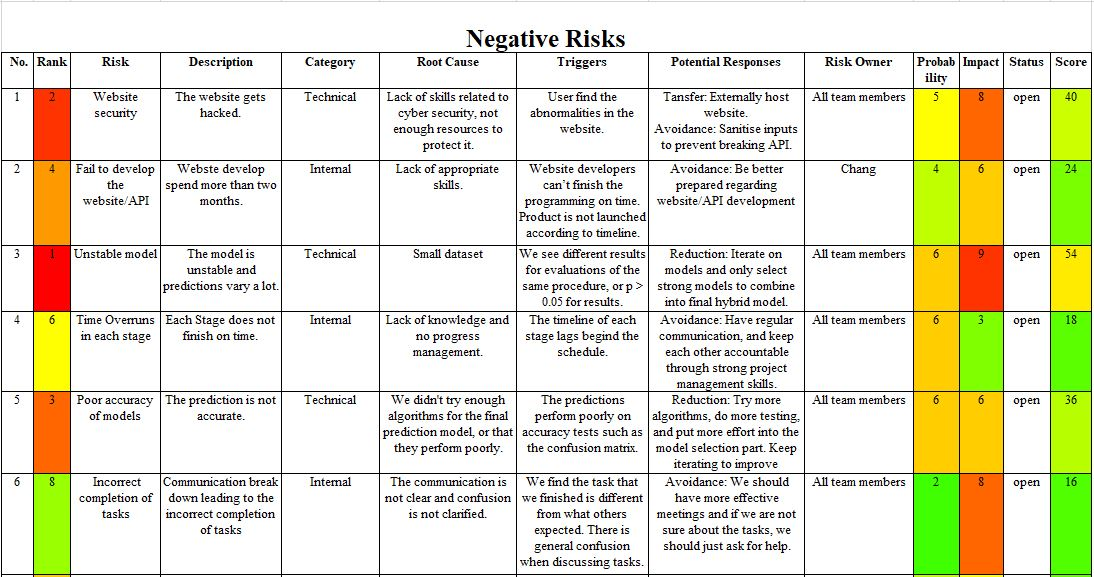
\includegraphics[width=1.5\textwidth]{RiskRegister1.jpg}
\end{figure}
\end{landscape}
\begin{landscape}
\begin{figure}
    \centering
    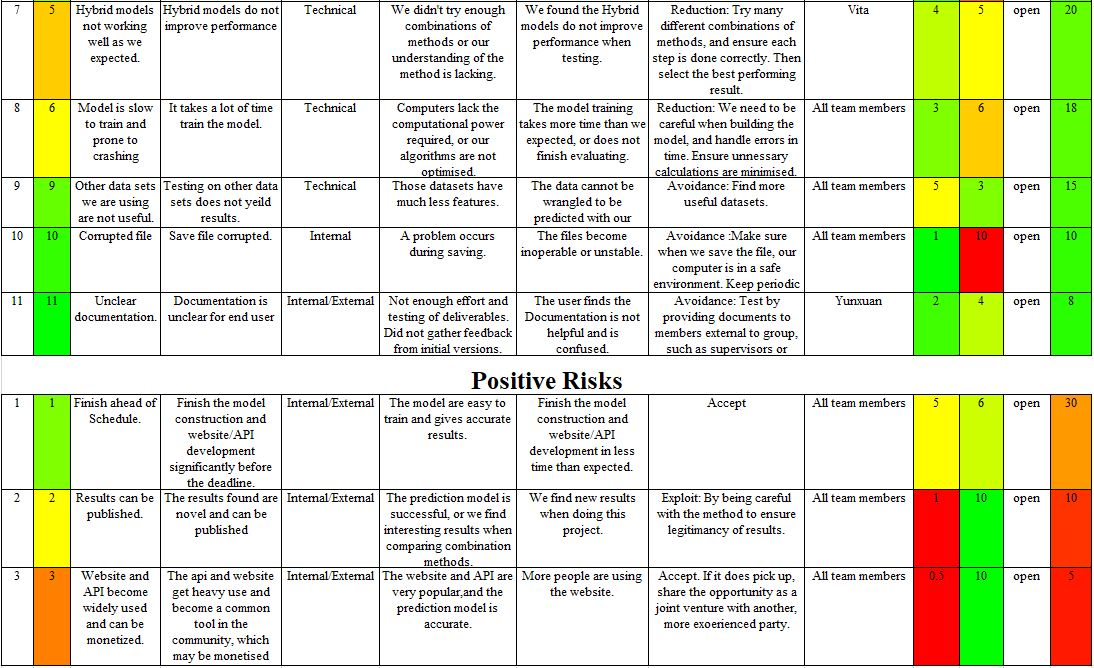
\includegraphics[width=1.5\textwidth]{RiskRegister2.jpg}
    \label{fig:Risk}
    \caption{Risk Register, detailing both positive and negative risks.}
\end{figure}
\end{landscape}


%Work Breakdown Structure table:https://app.lucidchart.com/invitations/accept/7d7b42bb-c508-4179-b039-d63243aded89
\begin{landscape}
\subsection{Work Breakdown Structure}
\begin{figure}[h!]
    \centering
    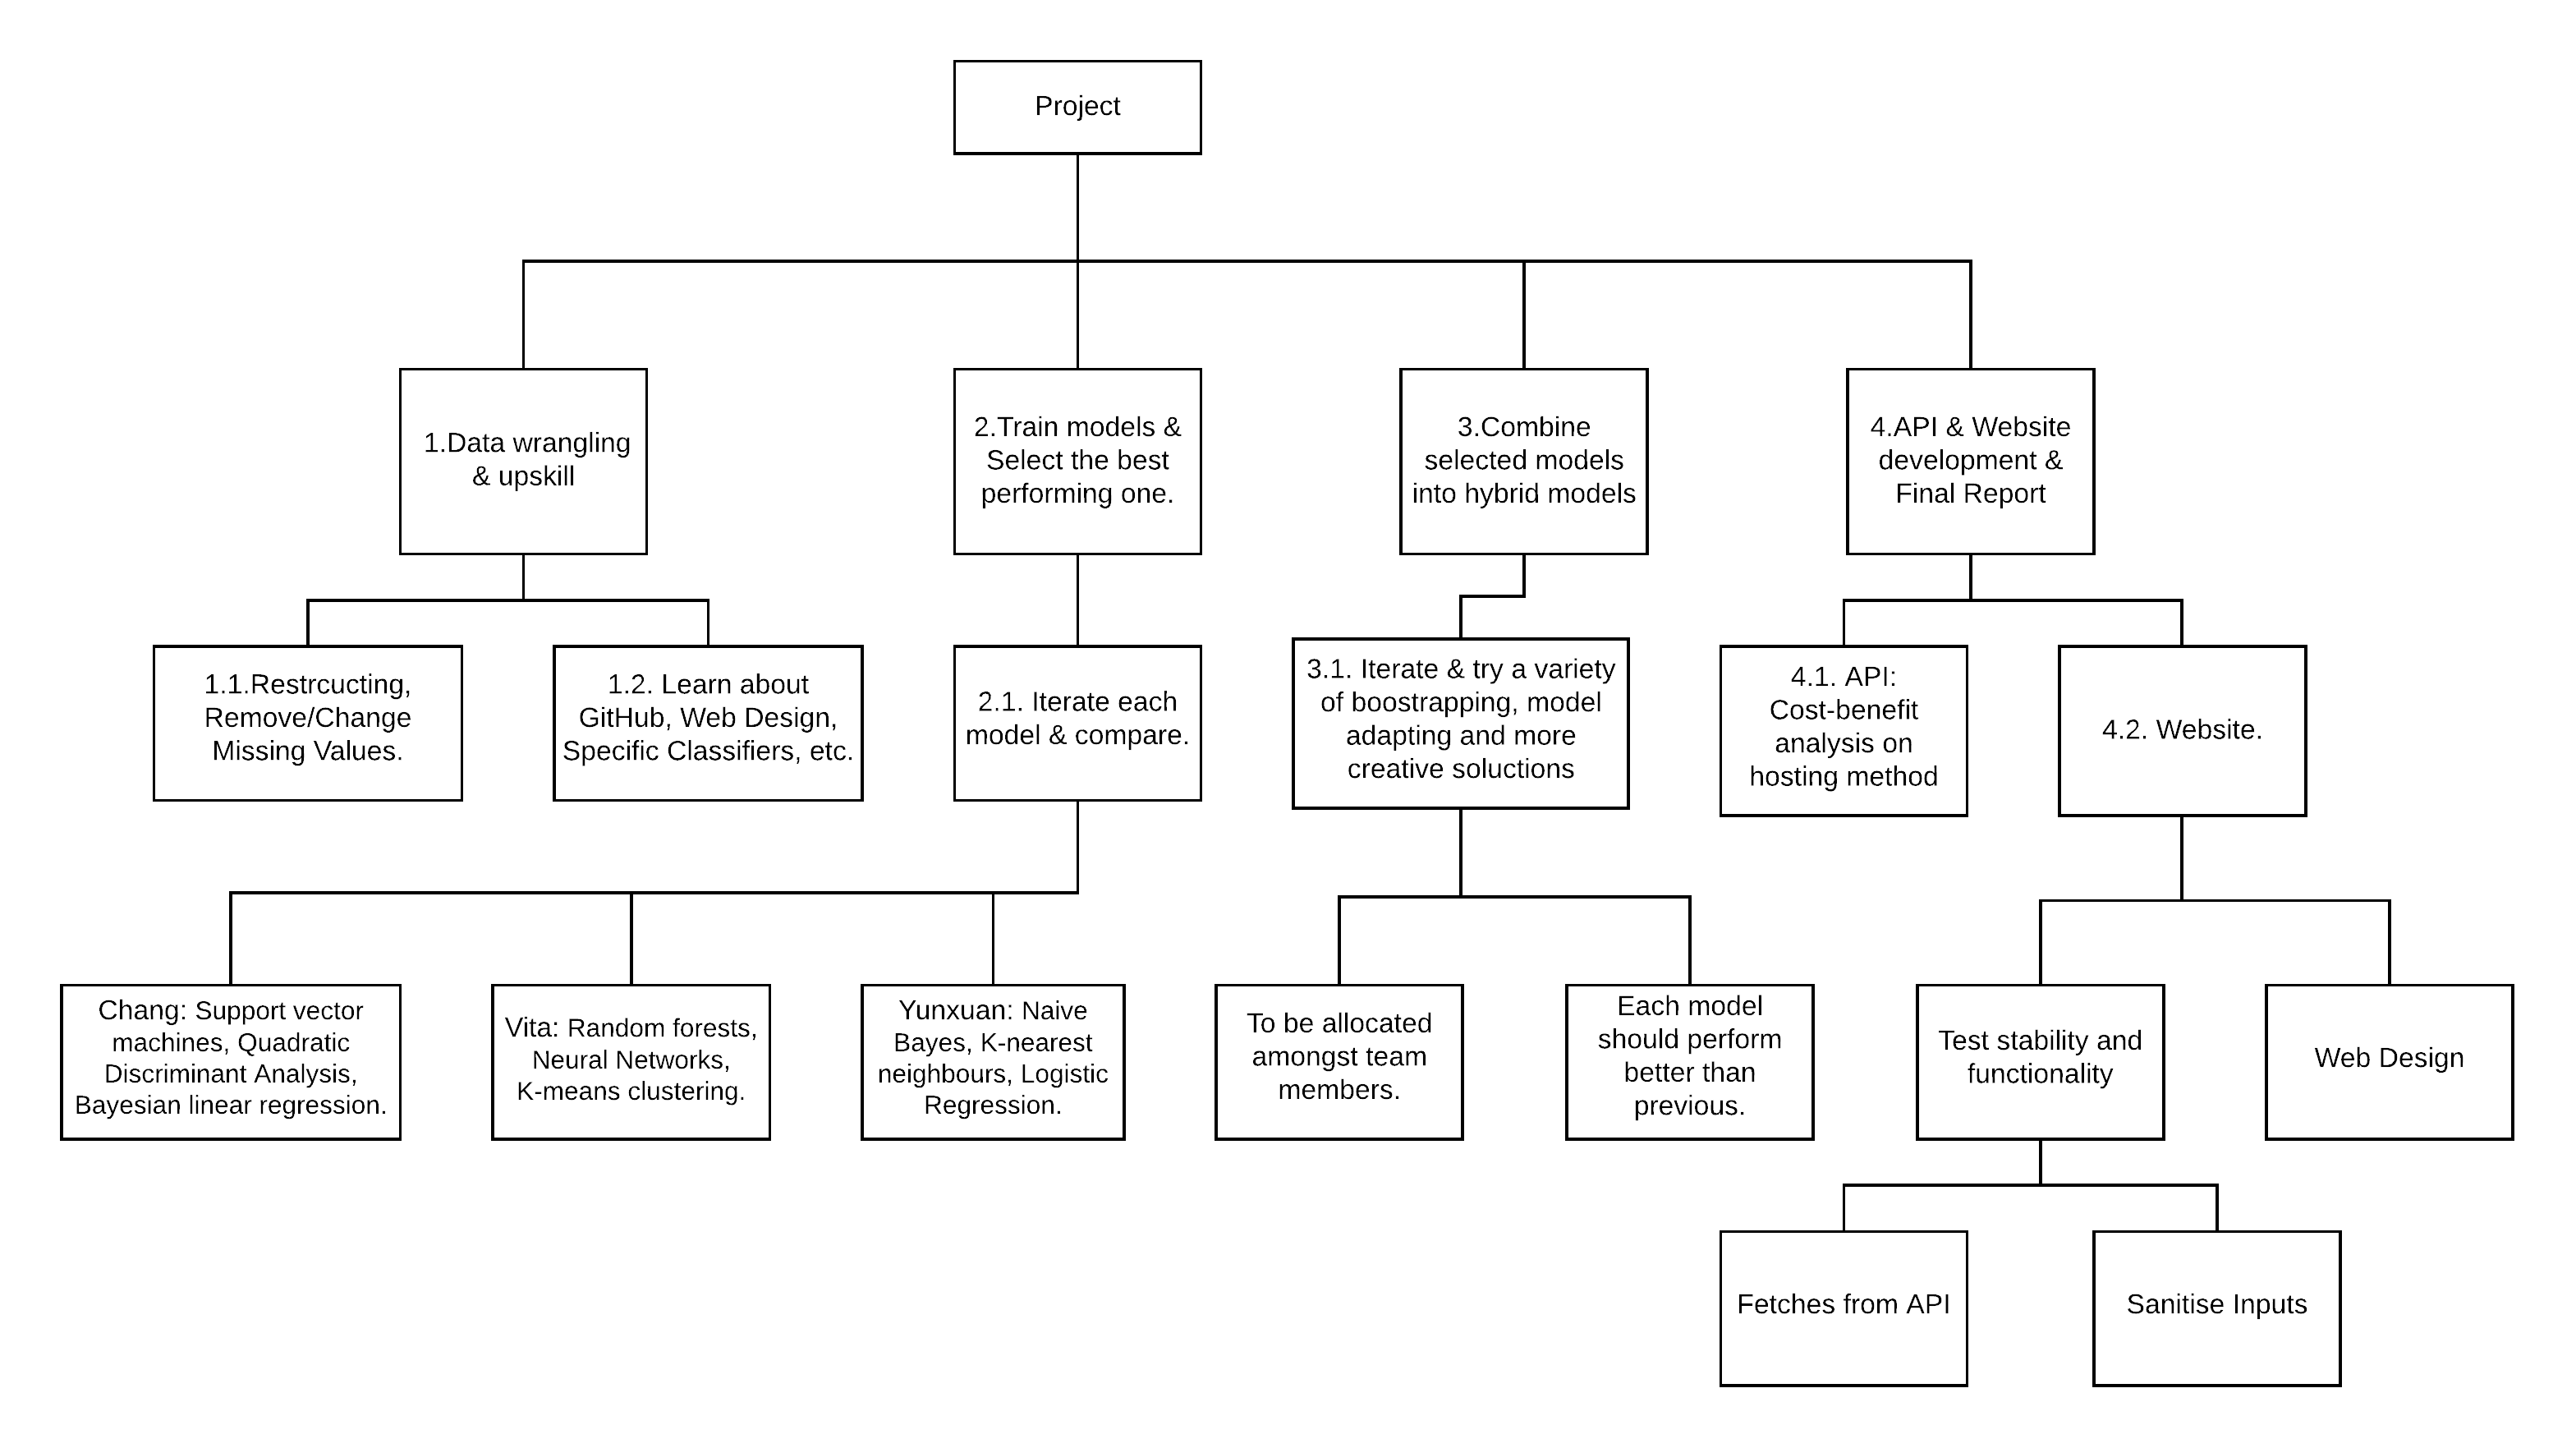
\includegraphics[width=1.5\textwidth]{Work Breakdown.png}
    \caption{Work Breakdown Structure, separated by stage.}
    \label{fig:WBS}
\end{figure}
\end{landscape}

\subsection{Dependencies Table}
\begin{figure}[ht] 
    \centering
    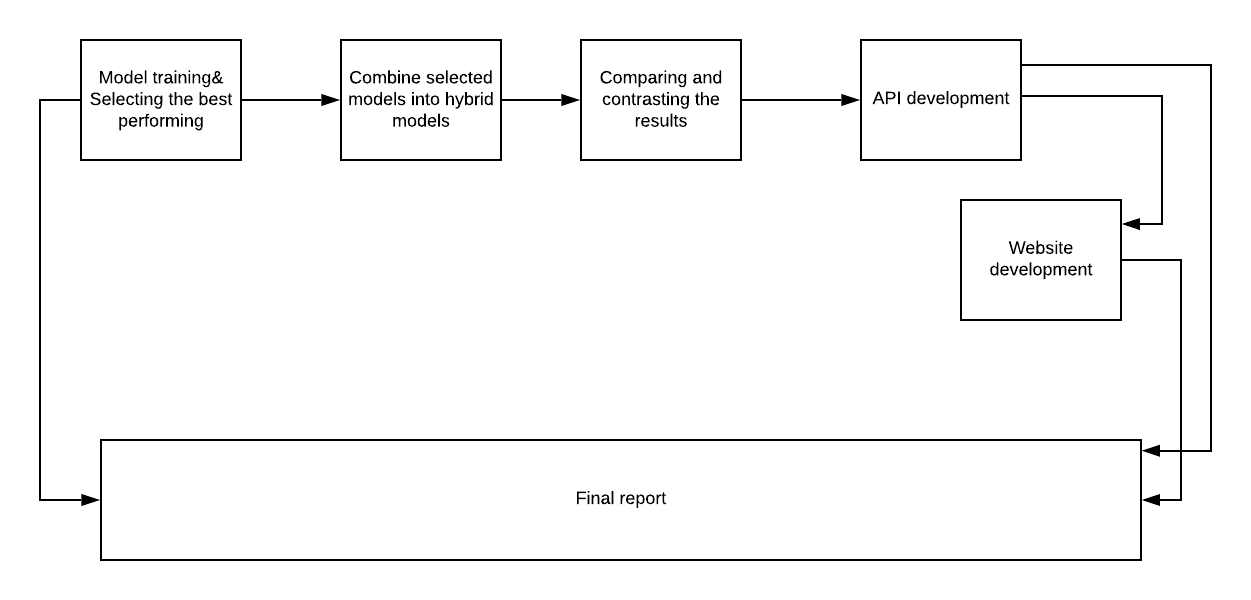
\includegraphics[width=0.8\textwidth]{Dependencies Table.png}
    \caption{A dependencies table, or network diagram, summarising the key stages of the project. Note the use of arrows specifying the specific dependancy between events.}
    \label{fig:dependency}
\end{figure}
%Dependency table:https://app.lucidchart.com/invitations/accept/6979a3e2-c31d-4986-bbb1-1477c9caedcc

\subsection{Packages Required}
    \begin{itemize}
    \item API hosting: plumber
    \item Naive Bayes: h2o,naibebayes 
    \item Logistic Regression: glmnet
    \item Support Vector Machines: e1071, pathClass, penalizedSVM
    \item Decision Tree: tree, rpart
    \item Neural Network: nnet, neuralnet, brnn
    \item Random Forest: randomForest
    \item Boosting: mboost, xgboost
    \item K-nearest Neighbours: knn(function)
    \item Stepwise regression: leaps
    \item Gaussian Processes: GauPro
    \item Bayesian Linear Regression: BLR
    \item LDA/QDA: MASS
    \end{itemize}
    
\subsection{Team Member's Contribution}
\begin{itemize}
\item Chang: Methodology, Test Planning, the first three parts of the project management plan (3.1 - 3.3), and proof reading.
\item Vita: Literature Review, sections of Methodology and Test Planning.
\item Yunxuan: External Design, the last two parts of the project management plan (3.4 - 3.5), and all diagrams.
\end{itemize}
\end{document}
%%TC:endignore
%end{docume\dont}